\documentclass[twoside]{article}

\usepackage{epsfig}
\usepackage{float}
\usepackage{amsmath,amsthm,amssymb,enumerate,mdwlist}
\setlength{\oddsidemargin}{0.25 in}
\setlength{\evensidemargin}{-0.25 in}
\setlength{\topmargin}{-0.6 in}
\setlength{\textwidth}{6.5 in}
\setlength{\textheight}{8.5 in}
\setlength{\headsep}{0.75 in}
\setlength{\parindent}{0 in}
\setlength{\parskip}{0.1 in}

\newcommand{\lecture}[3]{
   \pagestyle{myheadings}
   \thispagestyle{plain}
   \newpage
   \setcounter{page}{1}
   \noindent
   \begin{center}
   \framebox{
      \vbox{\vspace{2mm}
    \hbox to 6.28in { {\bf 10-708:~Probabilistic Graphical Models
10-708, Spring 2013 \hfill} }
       \vspace{6mm}
       \hbox to 6.28in { {\Large \hfill #1  \hfill} }
       \vspace{6mm}
       \hbox to 6.28in { {\it Lecturer: #2 \hfill Scribes: #3} }
      \vspace{2mm}}
   }
   \end{center}
   \markboth{#1}{#1}
   \vspace*{4mm}
}

\begin{document}

\lecture{Monte Carlo Methods}{Eric P. Xing}{Willie Neiswanger and Xiaohua Yan} % Lecture name, Lecturer, Scribes
\section{Introduction}
Previous lectures covered both exact inference algorithms (variable elimination, message passing, junction tree algorithm), and approximate inference algorithms (loopy belief propagation, mean field approximation). This lecture introduces an additional class of approximate inference algorithms known as stochastic simulation or sampling methods.

The basic motivation behind these methods stems from the problem that, for a random variable $X \sim P(x)$, it may be hard to find a closed form expression for $P(x)$ or for other related quantities of interest such as $\mathbb{E}[g(X)]$. A potential solution involves using samples $z_1,\ldots,z_N \sim P(x)$ to estimate quantities of interest, for example with 
\begin{equation*}
    \mathbb{E}[g(X)] \approx \frac{1}{N} \sum_{i=1}^N g(z_i)
\end{equation*}
This task is further complicated in cases where we only have access to an unnormalized distribution $P^*(x)$, where $P(x) = \frac{1}{Z} P^*(x)$. The following sections cover a collection of methods for drawing samples from a distribution or for using random draws to compute quantities of interest.

\section{Naive Sampling}
In order to draw samples from a target distribution, one intuition is that we could directly draw different samples uniformly from the state space and evaluate $P^*(\mathbf{x})$ at these points. However, even though the samples can be easily evaluated for $P^*(\mathbf{x})$, it might still work poorly on high-dimensional distributions. To see why this is the case, consider the following \textit{alarm example}, and the table on the right displays 10 samples drawn according to the probabilities given in the BN, where 1 denotes \textit{true} and 0 denotes \textit{false}:
\begin{figure}[H]
\minipage{0.5\textwidth}
\begin{center}
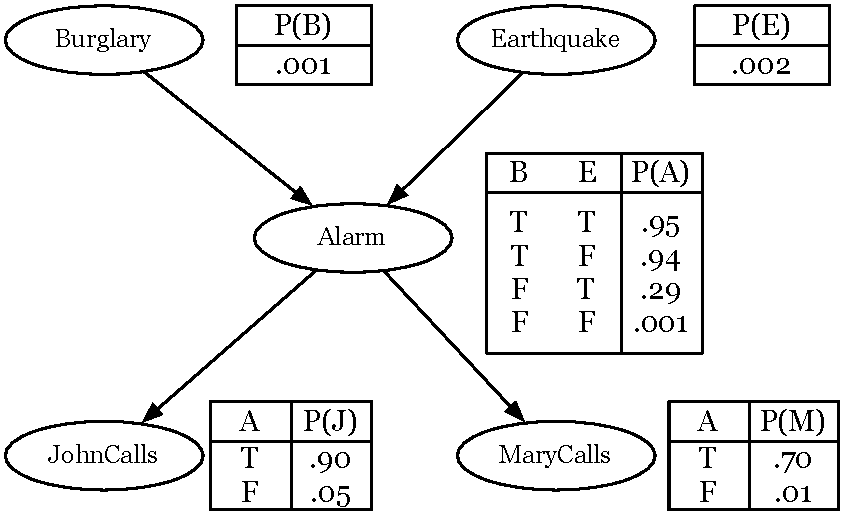
\includegraphics[scale=0.5]{alarm_example}
\end{center}
\endminipage\hfill
\minipage{0.5\textwidth}
\begin{center}
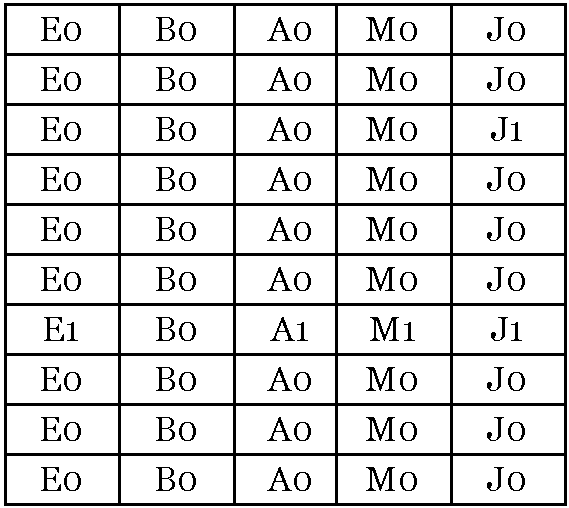
\includegraphics[scale=0.5]{alarm_table}
\end{center} 
\endminipage\hfill \\
\end{figure}
As can be observed from the example, if we want to compute $P(J|B1)$ according to the samples, the result would be $P(J|A1) = P(J,A1)/P(B1)= <0,1>$, since there is only one sample available. A more extreme case would be to compute $P(J|A1)=P(J,B1)/P(B1)$, which is not defined because there is no such sample available. Therefore, we can imagine that for a model with hundreds or more variables, rare events will be very hard to garner enough samples even after a long time of sampling.

\section{Rejection Sampling}
Suppose we want samples $z_1,\ldots,z_N \sim P(x)$, but only have access to the unnormalized distribution $P^*(x)$. In order to use rejection sampling to draw $z_1,\ldots,z_N$, we make use of a proposal distribution $q(x)$ that satisfies $P^*(x) \leq Mq(x)$ for all $x$ and for some $M>0$. We must define $q(x)$, and choose it to be a distribution from which we can easily draw samples. 

Once we have defined a $q(x)$, rejection sampling proceeds as follows:
\begin{enumerate*}
    \item Initialize $i=1$
    \item While $i \leq N$
    \begin{enumerate*}
        \item Sample $x \sim q(x)$ and $u \sim \text{Unif}(0,1)$
        \item If $u < \frac{P^*(x)}{Mq(x)}$
        \begin{enumerate*}
            \item $z_i = x$
            \item $i = i+1$
        \end{enumerate*}
    \end{enumerate*}
\end{enumerate*}

The main problem with rejection sampling is that a high percentage of the samples may be rejected, making it hard to efficiently attain a useful number of samples or to estimate desired quantities. This is especially problematic when $P(x)$ is a distribution over a high dimensional set, which can cause the acceptance percentage to plummet.

\section{Importance Sampling}
Importance sampling is \textit{not} a method for generating samples from the target density $P(\mathbf{x})$. Rather, it estimates the expectation of a function $\phi(x)$. Importance sampling deploys a simpler proposal distribution $Q(x)$ from which we can generate samples and satisfies the condition that $Q(x)>0$ whenever $P(x)>0$. In importance sampling, we generate $M$ samples from $Q(x)$ and suppose we can evaluate the samples for the unnormalized version of $P(x)$. For each sample, define
\[w^{(m)}=\frac{P(x^{(m)})}{Q(x^{(m)})}\]
Then the importance weighted estimator is
\begin{align*}
\hat{\Phi}(x) &=\int \phi(x)P(x)dx\\
&=\int \phi(x)\frac{P(x)}{Q(x)}Q(x)dx\\
&\simeq \frac{1}{M}\sum_m\phi(x^{(m)})\frac{P(x^{(m)})}{Q(x^{(m)})}\\
&=\frac{1}{M}\sum_m\phi(x^{(m)})w^{(m)}
\end{align*}
The unnormalized version of estimator is unbiased because we have
\[E_Q[\phi(x)w(x)]=\int \phi(x)w(x)Q(x)dx=\int \phi(x)\frac{P(x)}{Q(x)}Q(x)dx=E_P(\phi(x))\]
Suppose we can only evaluate $P^*(x)=\alpha P(x)$ instead of $P(x)$. To get around the normalization constant $\alpha$, first define
\[r(x)=\frac{P^*(x)}{Q(x)}\]
then our estimator can be derived as follows:
\begin{align*}
\hat{\Phi}(x) &= \int\phi(x)P(x)dx\\
&=\frac{1}{\alpha}\int \phi(x)\frac{P^*(x)}{Q(x)}Q(x)dx\\
&=\frac{\int \phi(x)r(x)Q(x)dx}{\int r(x)Q(x)dx}\\
&\simeq \frac{\sum_m\phi(x^{(m)})r^{(m)}}{\sum_mr^{(m)}}\\
&=\sum_m\phi(x^{(m)})w^{(m)}, \text{where } w^{(m)}=\frac{r^{(m)}}{\sum_mr^{(m)}}
\end{align*}
This importance weighted estimator is biased. For example, suppose $M=1$, then
\[E_Q[\frac{\phi(x^{(1)})r(x^{(1)})}{r(x^{(1)})}]=\int \phi(x)Q(x)dx=E_Q(\phi(x))\neq E_P(\phi(x))\]
However, the normalized importance sampling is asymptotically unbiased, and the variance of the normalized importance sampler is usually lower in practice. Also, it is common that we can evaluate $P^*(x)$ but not $P(x)$ (e.g. $P(x|e)=P^*(x)/P(e)$ for Bayes net, and $P(x)=P^*(x)/Z$ for MRF).

\section{Weighted Resampling}
Importance sampling can run into problems when the proposal distribution $Q(x)$ is dissimilar from the target distribution $P(x)$. To remedy this problem, weighted resampling involves carrying out a secondary sampling step where we redraw from the set of samples based on their computed weights.

In particular, importance sampling with resampling, also known as sampling importance resampling (SIR), can be used to to approximately sample $z^{(1)},\ldots,z^{(N)} \sim P(x)$. SIR involves the following steps:
\begin{enumerate*}
    \item Draw $x^{(1)},\ldots,x^{(N)} \sim Q(x)$, for some proposal $Q(x)$
    \item Compute sample weights $w_1,\ldots,w_N$, where $w_i = \frac{r^i}{\sum_i r^i}$
    \item Draw $a_1,\ldots,a_N \sim \text{Cat}(w_1,\ldots,w_N)$ 
    \item Set $z^{(i)} = x^{(a_i)}$ for $i = 1,\ldots,N$
\end{enumerate*}

\begin{figure*}[!tbp]
  \centering
  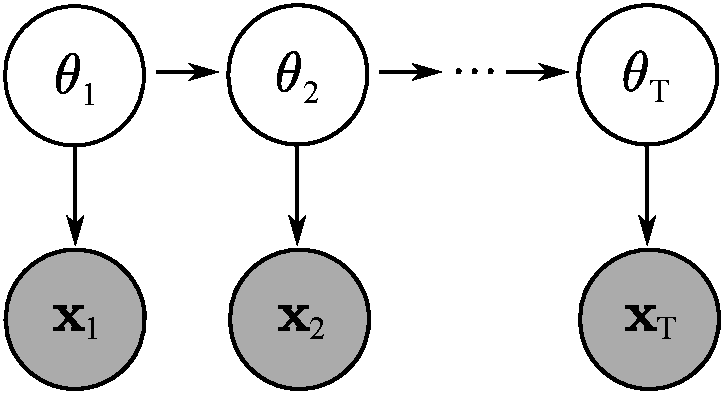
\includegraphics[width=0.3\textwidth]{dynamicBayesNet.pdf}
  \caption{An example sequential Bayesian model, with latent variables $\theta_1,\ldots,\theta_T$ and observations $x_1,\ldots,x_T$.}
  \label{fig:dynamicBayesNet}
\end{figure*}

A particle filter, also known as a sequential Monte Carlo (SMC) method, is a special type of SIR that can be viewed as a sequential version of importance sampling with resampling. In sequential Bayesian models (an example of which is shown in Figure~\ref{fig:dynamicBayesNet}) a particle filter allows one to draw samples $z_{1:T}^{(1)},\ldots,z_{1:T}^{(M)}$ from the posterior $P(\theta_{1:T} | x_{1:T})$ (i.e. the posterior over the latent variables given the observations) by sequentially building samples of the form $z_{1:t}^{(1)},\ldots,z_{1:t}^{(M)} \sim P(\theta_{1:t} | x_{1:t})$, for $t=1,\ldots,T$. This procedure can be written as follows: 
\begin{enumerate*}
    \item At each time step $t=1,\ldots,T$
    \begin{enumerate*}
        \item For each particle $m = 1,\ldots,M$
        \begin{enumerate*}
            \item Draw $z_t^{(m)} \sim Q(\theta_t | \theta_{t-1}, x_t)$ for some proposal distribution $Q(\cdot|\theta_{t-1},x_t)$
            \item Compute particle weight $\tilde{w}_t^{(m)} = w_{t-1}^{(m)} \times \frac{P(x_t | z_t^{(m)}) P(z_t^{(m)}|z_{t-1}^{(m)})}{Q(z_t^{(m)} | z_{t-1}^{(m)}, x_t)}$
        \end{enumerate*}
        \item Normalize the weights $w_t^{(m)} = \frac{\tilde{w}_t^{(m)}}{\sum_m \tilde{w}_t^{(m)}}$
        \item For each particle $m$, resample $z_t^{(m)}$ from $z_t^{(1)},\ldots,z_t^{(M)}$ with probability proportional to their weights.
    \end{enumerate*}
\end{enumerate*}

\section{Rao-Blackwellised Sampling}
So far we have pointed out that sampling in high dimensional spaces can cause high variance in the estimate. The Rao-Blackwell theorem can be stated as follows:

\textbf{Rao-Blackwell Theorem:} Let $\hat{\theta}$ be an estimator, and $T$ a sufficient statistic, both for $\theta$. Then the estimator $\hat{\theta}^*(X_1,...,X_n)=E(\hat{\theta}(X_1,...,X_n)|T(X_1,...,X_n))$ is at least as good as $\hat{\theta}$ in terms of mean squared errors.

Such idea can be applied to sampling. Namely, first we sample some variables $X_p$, and conditional on that, we can compute the expected value of the rest variables $X_d$ analytically:
\begin{align*}
E_{P(X|e)}[f(X)] &= \int p(x_p,x_d|e)f(x_p,x_d)dx_pdx_d\\
&=\int_{x_p}p(x_p|e)\left(\int_{x_d}p(x_d|x_p,e)f(x_p,x_d)dx_d\right)dx_p\\
&=\int_{x_p}p(x_p|e)E_{p(X_d|x_p,e)}[f(x_p,X_d)]dx_p\\
&=\frac{1}{M}\sum_mE_{p(X_d|x_p^{(m)},e)}[f(x_p^{(m)},X_d)]
\end{align*}
This estimator has lower variance, because the following equation holds:
\[\text{var}[\tau(X_p,X_d)]=\text{var}[E[\tau(X_p,X_d)|X_p]]+E[\text{var}[\tau(X_p,X_d)|X_p]]\]
And hence $E[\text{var}[\tau(X_p,X_d)|X_p]]\leq\text{var}[\tau(X_p,X_d)]$.
\end{document}

